\documentclass{article}
\usepackage{../assignment_preamble}

\title{Homework 6}
\author{Ravi Kini}
\date{November 12, 2025}

\begin{document}

\maketitle

\problem{}
The following tree represents the possible outcomes of flipping a coin with a bias of $\theta = 0.3$ five times:
\begin{center}
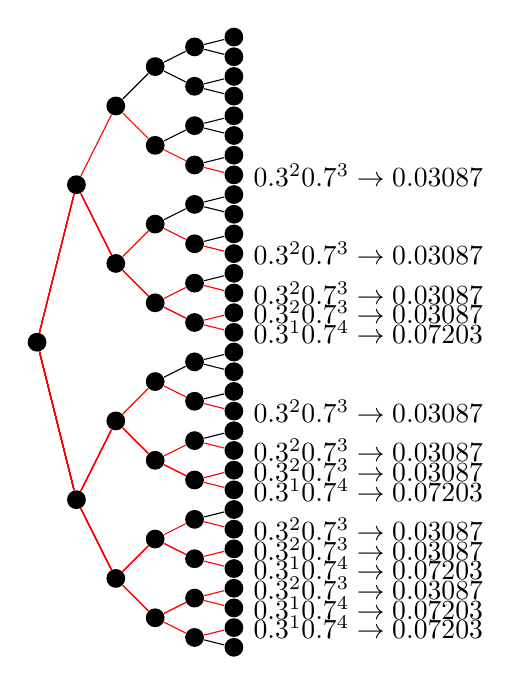
\begin{tikzpicture}[scale=0.5,
       dot/.style = {circle, fill, inner sep=2.4pt, node contents={},
                     label=#1},
every edge/.style = {draw, postaction=decorate}
                        ]
\node (hhhhh) at (0,0) [dot=right:];
\node (hhhht) at (0,-0.5) [dot=right:];
\node (hhhth) at (0,-1) [dot=right:];
\node (hhhtt) at (0,-1.5) [dot=right:];
\node (hhthh) at (0,-2) [dot=right:];
\node (hhtht) at (0,-2.5) [dot=right:];
\node (hhtth) at (0,-3) [dot=right:];
\node (hhttt) at (0,-3.5) [dot=right:$0.3^20.7^3 \to 0.03087$];
\node (hthhh) at (0,-4) [dot=right:];
\node (hthht) at (0,-4.5) [dot=right:];
\node (hthth) at (0,-5) [dot=right:];
\node (hthtt) at (0,-5.5) [dot=right:$0.3^20.7^3 \to 0.03087$];
\node (htthh) at (0,-6) [dot=right:];
\node (httht) at (0,-6.5) [dot=right:$0.3^20.7^3 \to 0.03087$];
\node (httth) at (0,-7) [dot=right:$0.3^20.7^3 \to 0.03087$];
\node (htttt) at (0,-7.5) [dot=right:$0.3^10.7^4 \to 0.07203$];
\node (thhhh) at (0,-8) [dot=right:];
\node (thhht) at (0,-8.5) [dot=right:];
\node (thhth) at (0,-9) [dot=right:];
\node (thhtt) at (0,-9.5) [dot=right:$0.3^20.7^3 \to 0.03087$];
\node (ththh) at (0,-10) [dot=right:];
\node (ththt) at (0,-10.5) [dot=right:$0.3^20.7^3 \to 0.03087$];
\node (thtth) at (0,-11) [dot=right:$0.3^20.7^3 \to 0.03087$];
\node (thttt) at (0,-11.5) [dot=right:$0.3^10.7^4 \to 0.07203$];
\node (tthhh) at (0,-12) [dot=right:];
\node (tthht) at (0,-12.5) [dot=right:$0.3^20.7^3 \to 0.03087$];
\node (tthth) at (0,-13) [dot=right:$0.3^20.7^3 \to 0.03087$];
\node (tthtt) at (0,-13.5) [dot=right:$0.3^10.7^4 \to 0.07203$];
\node (ttthh) at (0,-14) [dot=right:$0.3^20.7^3 \to 0.03087$];
\node (tttht) at (0,-14.5) [dot=right:$0.3^10.7^4 \to 0.07203$];
\node (tttth) at (0,-15) [dot=right:$0.3^10.7^4 \to 0.07203$];
\node (ttttt) at (0,-15.5) [dot=right:];

\node (hhhh) at (-1, -0.25) [dot=right:];
\node (hhht) at (-1, -1.25) [dot=right:];
\node (hhth) at (-1, -2.25) [dot=right:];
\node (hhtt) at (-1, -3.25) [dot=right:];
\node (hthh) at (-1, -4.25) [dot=right:];
\node (htht) at (-1, -5.25) [dot=right:];
\node (htth) at (-1, -6.25) [dot=right:];
\node (httt) at (-1, -7.25) [dot=right:];
\node (thhh) at (-1, -8.25) [dot=right:];
\node (thht) at (-1, -9.25) [dot=right:];
\node (thth) at (-1, -10.25) [dot=right:];
\node (thtt) at (-1, -11.25) [dot=right:];
\node (tthh) at (-1, -12.25) [dot=right:];
\node (ttht) at (-1, -13.25) [dot=right:];
\node (ttth) at (-1, -14.25) [dot=right:];
\node (tttt) at (-1, -15.25) [dot=right:];

\node (hhh) at (-2, -0.75) [dot=right:];
\node (hht) at (-2, -2.75) [dot=right:];
\node (hth) at (-2, -4.75) [dot=right:];
\node (htt) at (-2, -6.75) [dot=right:];
\node (thh) at (-2, -8.75) [dot=right:];
\node (tht) at (-2, -10.75) [dot=right:];
\node (tth) at (-2, -12.75) [dot=right:];
\node (ttt) at (-2, -14.75) [dot=right:];

\node (hh) at (-3, -1.75) [dot=right:];
\node (ht) at (-3, -5.75) [dot=right:];
\node (th) at (-3, -9.75) [dot=right:];
\node (tt) at (-3, -13.75) [dot=right:];

\node (h) at (-4, -3.75) [dot=right:];
\node (t) at (-4, -11.75) [dot=right:];

\node (_) at (-5, -7.75) [dot=right:];
%
\path
(hh) edge (hhh)
(hhh) edge (hhhh) edge (hhht)
(hht) edge (hhth)
(hth) edge (hthh)
(thh) edge (thhh)
(hhhh) edge (hhhhh) edge (hhhht)
(hhht) edge (hhhth) edge (hhhtt)
(hhth) edge (hhthh) edge (hhtht)
(hhtt) edge (hhtth)
(hthh) edge (hthhh) edge (hthht)
(htht) edge (hthth)
(htth) edge (htthh)
(thhh) edge (thhhh) edge (thhht)
(thht) edge (thhth)
(thth) edge (ththh)
(tthh) edge (tthhh)
(tttt) edge (ttttt)
;
\path[draw=red]
(_) edge (h) (h) edge (ht) (ht) edge (htt) (htt) edge (httt) (httt) edge (htttt)
(_) edge (h) (h) edge (hh) (hh) edge (hht) (hht) edge (hhtt) (hhtt) edge (hhttt)
(_) edge (h) (h) edge (ht) (ht) edge (hth) (hth) edge (htht) (htht) edge (hthtt)
(_) edge (h) (h) edge (ht) (ht) edge (htt) (htt) edge (htth) (htth) edge (httht)
(_) edge (h) (h) edge (ht) (ht) edge (htt) (htt) edge (httt) (httt) edge (httth)
(_) edge (t) (t) edge (th) (th) edge (thh) (thh) edge (thht) (thht) edge (thhtt)
(_) edge (t) (t) edge (th) (th) edge (tht) (tht) edge (thtt) (thtt) edge (thttt)
(_) edge (t) (t) edge (th) (th) edge (tht) (tht) edge (thth) (thth) edge (ththt)(_) edge (t) (t) edge (th) (th) edge (tht) (tht) edge (thtt) (thtt) edge (thtth)
(_) edge (t) (t) edge (tt) (tt) edge (tth) (tth) edge (ttht) (ttht) edge (tthtt)
(_) edge (t) (t) edge (tt) (tt) edge (tth) (tth) edge (tthh) (tthh) edge (tthht)
(_) edge (t) (t) edge (tt) (tt) edge (tth) (tth) edge (ttht) (ttht) edge (tthth)
(_) edge (t) (t) edge (tt) (tt) edge (ttt) (ttt) edge (ttth) (ttth) edge (ttthh)
(_) edge (t) (t) edge (tt) (tt) edge (ttt) (ttt) edge (ttth) (ttth) edge (tttht)
(_) edge (t) (t) edge (tt) (tt) edge (ttt) (ttt) edge (tttt) (tttt) edge (tttth)
;
\end{tikzpicture}
\end{center}
The probability that the frequency deviates from the true bias by at most $\epsilon = 0.1$ is $0.03087 \cdot 10 + 0.07203 \cdot 5 = 0.66885$.

Using the formula:
\begin{align*}
    \sum_{x=1}^2 {5 \choose x} 0.3^x {(1 - 0.3)}^{5-x} & = {5 \choose 1} 0.3^1 0.7^4 + {5 \choose 2} 0.3^2 0.7^3 \\
    & = 0.66885
\end{align*}

\clearpage
\problem{}
The probability that the frequency of landing heads in $40$ tosses is $0.05$-close to the true bias of $1/4$ is:
\begin{align*}
    P_{1/4, 40}(|\text{frequency of landing heads} - 1/4| \leq 0.05) & = \sum_{x : \left|\frac{x}{40} - \frac{1}{4}\right| \leq 0.05} \text{Binom}_{1/4, 40}(x) \\
    & = \sum_{x=8}^{12} \text{Binom}_{1/4, 40}(x) \\
    & = \sum_{x=8}^{12} \frac{40!}{x!(40-x)!}\left(\frac{1}{4}\right)^x\left(\frac{3}{4}\right)^{40-x} \\
    & \approx 0.6389
\end{align*}

\clearpage
\problem{}
\begin{align*}
    0.95 & \leq 1 - \frac{1}{4n{(0.01)}^2} \\
    \frac{1}{4n{(0.01)}^2} & \leq 0.05 \\
    50000 & \leq n
\end{align*}
When estimating the bias of the coin by the observed frequency under the IID assumption, the estimation procedure has at least a $95\%$ probability of having an error less than $0.01$ when the coin is tossed at least $50000$ times.
\end{document}